\documentclass[12pt, a4paper]{article}
\usepackage{array}
\usepackage{graphicx}
\usepackage{longtable}
\usepackage{etoolbox}
\usepackage{subcaption}
\usepackage{float}
\usepackage{amsmath}
\usepackage{mathtools}

\newcommand*\mean[1]{\bar{#1}}

\setlength{\parindent}{0em}
\setlength{\parskip}{1em}

\newcounter{rowcntr}[table]
\renewcommand{\therowcntr}{\thetable.\arabic{rowcntr}}
% A new columntype to apply automatic stepping
\newcolumntype{N}{>{\refstepcounter{rowcntr}\therowcntr}c}
% Reset the rowcntr counter at each new tabular
\AtBeginEnvironment{tabular}{\setcounter{rowcntr}{0}}

\begin{document}

\tableofcontents
\pagebreak

\listoffigures
\listoftables
\pagebreak

\section{Background and Literature Review}
\subsection{Survey of online methods for changing and matching skin colour in Photoshop}
%TODO text
\pagebreak

\section{Methods}
To accomplish the objective of recolouring the skintone of a hand to a target colour, we wrote algorithms in C++ in Eclipse on OS X using OpenCV libraries. Eclipse is used to compile each iteration of the algorithm into an debug-mode excutable program named Recolor. For ease of testing, as the algorithm is modified, we add more functionality to the Recolor program and retain the ability to use previous versions of the algorithm. We use a custom Python script to run new versions of Recolor from the terminal to test it. All of the relevant code and its versions are hosted on a git repository at https://github.com/tiantianhan/recolor 

Recolor takes as input a hand image as well as a mask instructing it where to find the average skin colour of the hand, and a desired target skin colour. (Other flags and inputs are also used for testing purposes, see the Appendix for a full description of the usage.) Recolor then outputs the processed image where the skintone is adjusted to the target colour.

We iterated from simple to more complex algorithms, at each step testing the algorithm and evaluating the results. We tested progressive iterations on a set of hand images with varying skintones. The images are are shown in Figure \ref{img:input_hands_1}.

%all images that are not test results will be copied to the images folder

\begin{figure}[H]
    \centering
    \begin{subfigure}[b]{0.20\textwidth}
        \includegraphics[width=\textwidth]{images/hand_dark}
        \caption{}\label{img:input_hands_1_dark}
    \end{subfigure}
    ~
    \begin{subfigure}[b]{0.20\textwidth}
        \includegraphics[width=\textwidth]{images/hand_brown}
        \caption{}\label{img:input_hands_1_brown}
    \end{subfigure}
    ~
    \begin{subfigure}[b]{0.20\textwidth}
        \includegraphics[width=\textwidth]{images/hand_light}
        \caption{}\label{img:input_hands_1_light}
    \end{subfigure}
    ~
    \begin{subfigure}[b]{0.20\textwidth}
        \includegraphics[width=\textwidth]{images/hand_pale}
        \caption{}\label{img:input_hands_1_pale}
    \end{subfigure}
    \caption{Different hand images used for testing}\label{img:input_hands_1}
\end{figure}

 For each test, we called the Recolor program to transform the image of one hand to have the skintone of the hand in another image, then visually compared the processed image to the image of the target hand. We performed the process on all possible combinations of our test images, paying particular attention to the extreme cases, transforming from Figure \ref{img:input_hands_1_dark} to Figure \ref{img:input_hands_1_pale} and vice versa, as well as cases that start with a hand with midtone skin such as in Figure \ref{img:input_hands_1_brown} (as this is the most likely use case for applications that change a model's hand to match a range of skintones). We evaluated the resulting images subjectively, based on whether the processed hand looks believably like a hand naturally of that skintone, and noted any flaws that we then attempted to correct with the next iteration of the algorithm.

In the following subsections we summarize the results of each algorithm and our evaluation of the results.

\subsection{Simple brightness addition / subtraction}
\subsubsection{Algorithm}
To begin, we performed a simple addition of a value to each of the $rgb$ channels of the hand, such that the average colour of the hand in the processed image is equal to the average color of the hand in the target image. The algorithm is shown in Equation \ref{eq:boost_algo}.

\begin{equation} \label{eq:boost_algo}
r' = r + \delta_r
\end{equation}

Where 

\begin{equation*}
\delta_r = \mean{r_t} - \mean{r}
\end{equation*}

With the same equation applying for the $g$ and $b$ channels.

\subsubsection{Results}
The complete results are shown in Table \ref{tab:boost_test} in the Appendix, a portion is shown here for convenience.

\begin{longtable}{|c||c|c|c|}
    \caption*{Portion of test results of simple addition / subtraction brightening function from Table \ref{tab:boost_test} in the Appendix}\\
    \hline
    No. & Original & Target & Results \\ 
    \hline  \ref{row:boost_test_hand_brown_to_hand_dark} &
  \begin{minipage}{.29\textwidth}
    \includegraphics[width=\textwidth,height=\textheight,keepaspectratio]{../inputs/hand_brown.jpg}
  \end{minipage} & 
  \begin{minipage}{.29\textwidth}
    \includegraphics[width=\textwidth,height=\textheight,keepaspectratio]{../inputs/hand_dark.jpg}
  \end{minipage} & 
  \begin{minipage}{.29\textwidth}
    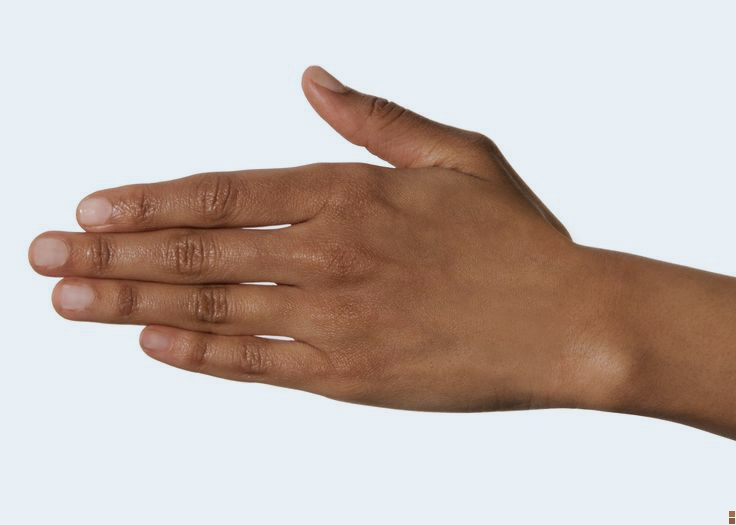
\includegraphics[width=\textwidth,height=\textheight,keepaspectratio]{../rc_test/outputs/20170516_boost_test/hand_brown_to_hand_dark.jpg}
  \end{minipage} \\
\hline  \ref{row:boost_test_hand_brown_to_hand_light} &
  \begin{minipage}{.29\textwidth}
    \includegraphics[width=\textwidth,height=\textheight,keepaspectratio]{../inputs/hand_brown.jpg}
  \end{minipage} & 
  \begin{minipage}{.29\textwidth}
    \includegraphics[width=\textwidth,height=\textheight,keepaspectratio]{../inputs/hand_light.jpg}
  \end{minipage} & 
  \begin{minipage}{.29\textwidth}
    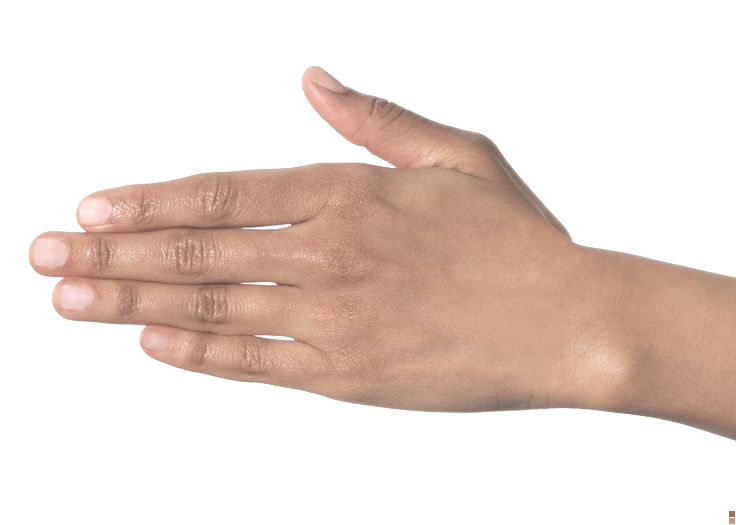
\includegraphics[width=\textwidth,height=\textheight,keepaspectratio]{../rc_test/outputs/20170516_boost_test/hand_brown_to_hand_light.jpg}
  \end{minipage} \\
  \hline  \ref{row:boost_test_hand_brown_to_hand_pale} &
  \begin{minipage}{.29\textwidth}
    \includegraphics[width=\textwidth,height=\textheight,keepaspectratio]{../inputs/hand_brown.jpg}
  \end{minipage} & 
  \begin{minipage}{.29\textwidth}
    \includegraphics[width=\textwidth,height=\textheight,keepaspectratio]{../inputs/hand_pale.jpg}
  \end{minipage} & 
  \begin{minipage}{.29\textwidth}
    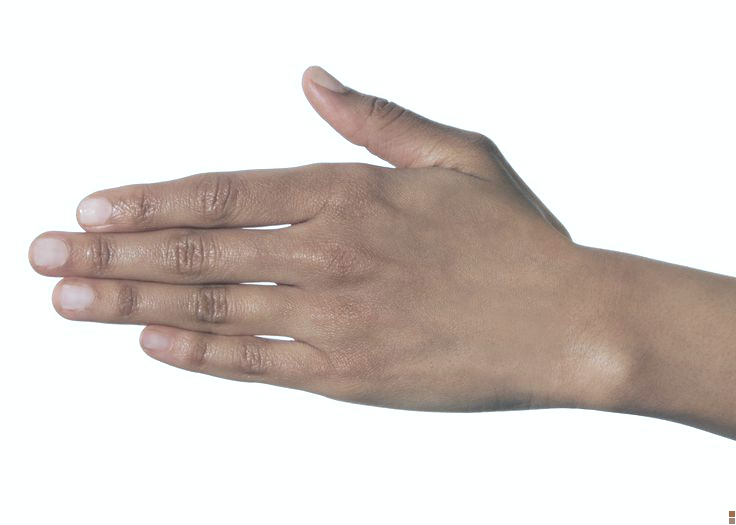
\includegraphics[width=\textwidth,height=\textheight,keepaspectratio]{../rc_test/outputs/20170516_boost_test/hand_brown_to_hand_pale.jpg}
  \end{minipage} \\
    \hline
\end{longtable}

\subsubsection{Evaluation}
Images of darker skintones and smaller changes between the original skintone and target colour to begin with (Row \ref{row:boost_test_hand_brown_to_hand_dark}) tend to have better results than images with large changes, especially towards lighter colours. This is likely because large changes force bright points in the original image to be truncated at white, and also causes dark regions on the image, such as shadows and grooves less close to true black, giving the image a ``high-key" look (Row \ref{row:boost_test_hand_brown_to_hand_light}).

In addition, we noted that at this stage the transformation from a dark coloured hand to a very pale hand, or even from a midtoned hand to a pale hand and vice versa is especially unconvincing. (Row \ref{row:boost_test_hand_brown_to_hand_pale}, also see \ref{row:boost_test_hand_dark_to_hand_pale} and \ref{row:boost_test_hand_pale_to_hand_dark})

\subsection{Proportional adjustment relative to average color}
\subsubsection{Algorithm}
To correct for the effect of the bright spots in the image image being over bright and the high-key appearance resulting from all the shadows being brightened, we used an algorithm that maps the black and white points of the image to the same value, and adjust the colors in between to match the target average colour. The algorithm is shown in Equation \ref{eq:prop_algo}.

\begin{equation} \label{eq:prop_algo}
  r' = \left.
  \begin{dcases}
    \displaystyle \Big(\frac{\mean{r_t}}{\mean{r}}\Big)r, & \text{for } r \leq \mean{r} \\
    \displaystyle 255 - 
    \Big(\frac{255 - \mean{r_t}}{255 - \mean{r}}\Big)(255 - r), & \text{for } r > \mean{r} \\
  \end{dcases}
  \right.
\end{equation}

With the same equation applying for the $g$ and $b$ channels.

\subsubsection{Results}
The complete results are shown in Table \ref{tab:prop_test} in the Appendix, a portion is shown here for convenience.

\begin{longtable}{|c||c|c|c|}
    \caption*{Portion of test results of adjusting proportionally based on distance of color to the average from Table \ref{tab:prop_test} in the Appendix}\\
    \hline
    No. & Original & Target & Results \\ 
    \hline  \ref{row:prop_test_hand_brown_to_hand_dark} &
  \begin{minipage}{.29\textwidth}
    \includegraphics[width=\textwidth,height=\textheight,keepaspectratio]{../inputs/hand_brown.jpg}
  \end{minipage} & 
  \begin{minipage}{.29\textwidth}
    \includegraphics[width=\textwidth,height=\textheight,keepaspectratio]{../inputs/hand_dark.jpg}
  \end{minipage} & 
  \begin{minipage}{.29\textwidth}
    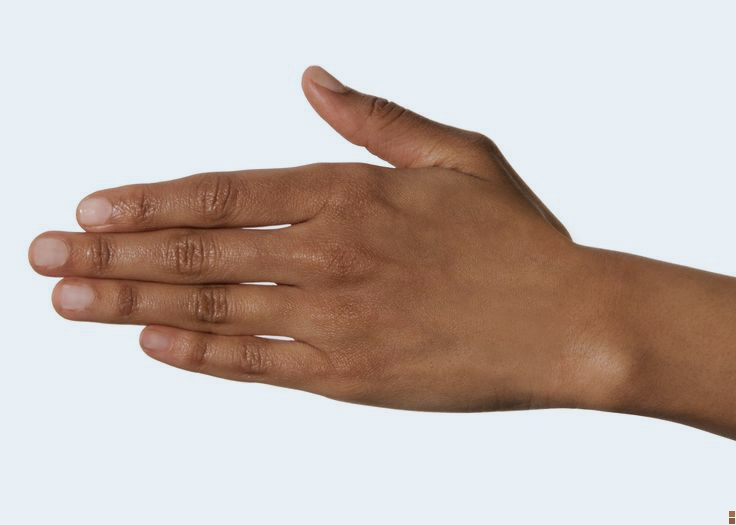
\includegraphics[width=\textwidth,height=\textheight,keepaspectratio]{../rc_test/outputs/20170516_boost_test/hand_brown_to_hand_dark.jpg}
  \end{minipage} \\
\hline  \ref{row:prop_test_hand_brown_to_hand_light} &
  \begin{minipage}{.29\textwidth}
    \includegraphics[width=\textwidth,height=\textheight,keepaspectratio]{../inputs/hand_brown.jpg}
  \end{minipage} & 
  \begin{minipage}{.29\textwidth}
    \includegraphics[width=\textwidth,height=\textheight,keepaspectratio]{../inputs/hand_light.jpg}
  \end{minipage} & 
  \begin{minipage}{.29\textwidth}
    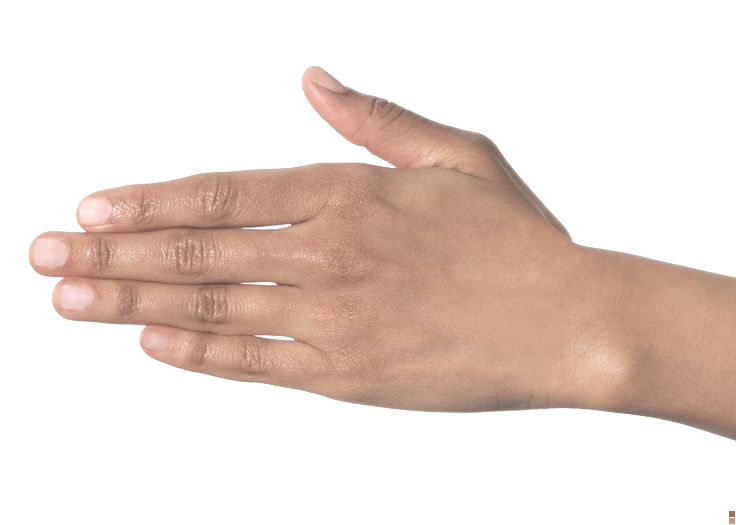
\includegraphics[width=\textwidth,height=\textheight,keepaspectratio]{../rc_test/outputs/20170516_boost_test/hand_brown_to_hand_light.jpg}
  \end{minipage} \\
  \hline  \ref{row:prop_test_hand_brown_to_hand_pale} &
  \begin{minipage}{.29\textwidth}
    \includegraphics[width=\textwidth,height=\textheight,keepaspectratio]{../inputs/hand_brown.jpg}
  \end{minipage} & 
  \begin{minipage}{.29\textwidth}
    \includegraphics[width=\textwidth,height=\textheight,keepaspectratio]{../inputs/hand_pale.jpg}
  \end{minipage} & 
  \begin{minipage}{.29\textwidth}
    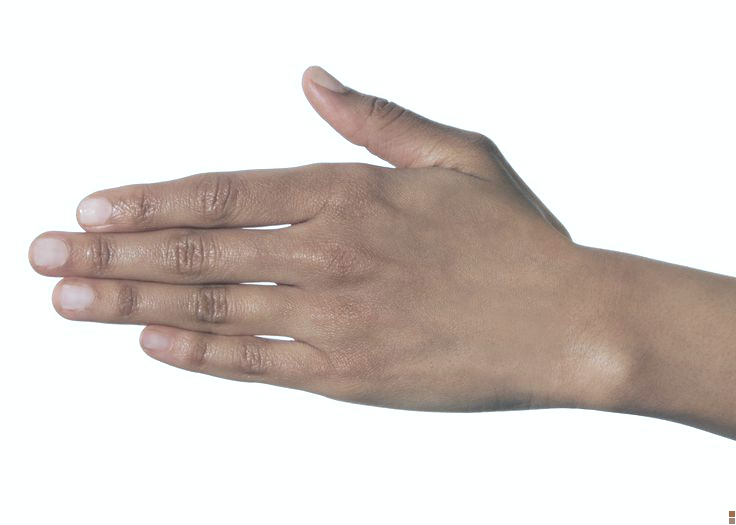
\includegraphics[width=\textwidth,height=\textheight,keepaspectratio]{../rc_test/outputs/20170516_boost_test/hand_brown_to_hand_pale.jpg}
  \end{minipage} \\
    \hline
\end{longtable}

\subsubsection{Evaluation}


\subsection{Proportional brightening with dark spot correction}
%TODO text
See Table \ref{tab:prop_correct_test} in the Appendix for full results.

\pagebreak

\appendix

\section{Appendix A}
\begin{longtable}{|N||c|c|c|}
	\caption{Test results of simple addition / subtraction brightening function.\label{tab:boost_test}}\\
	\hline
	\multicolumn{1}{|c||}{No.} & Original & Target & Results \\ 
	\hline
	    \label{row:boost_test_1} &
  \begin{minipage}{.29\textwidth}
    \includegraphics[width=\textwidth,height=\textheight,keepaspectratio]{../inputs/hand_dark.jpg}
  \end{minipage} & 
  \begin{minipage}{.29\textwidth}
    \includegraphics[width=\textwidth,height=\textheight,keepaspectratio]{../inputs/hand_pale.jpg}
  \end{minipage} & 
  \begin{minipage}{.29\textwidth}
    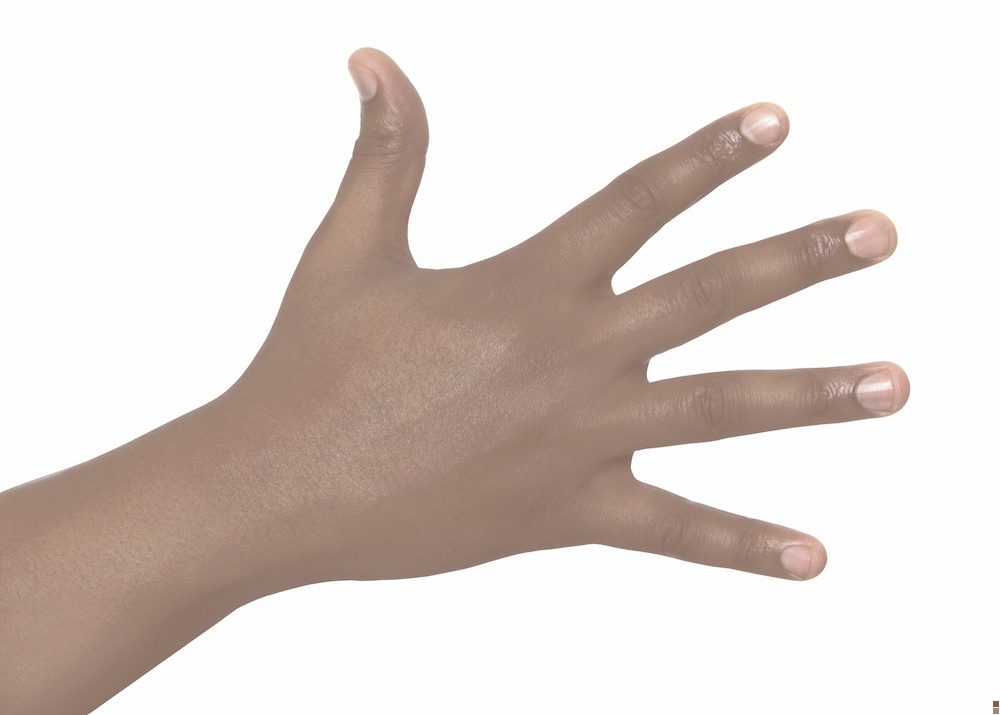
\includegraphics[width=\textwidth,height=\textheight,keepaspectratio]{../rc_test/outputs/debug/hand_dark_to_hand_pale.jpg}
  \end{minipage} \\
\hline
 \end{longtable}
\pagebreak
\begin{longtable}{|N||c|c|c|}
	\caption{Test results of brightening proportionally based on distance of color to the average.\label{tab:prop_test}}\\
	\hline
	\multicolumn{1}{|c||}{No.} & Original & Target & Results \\ 
	\hline
	    \label{row:prop_test_1} &
  \begin{minipage}{.29\textwidth}
    \includegraphics[width=\textwidth,height=\textheight,keepaspectratio]{../inputs/hand_dark.jpg}
  \end{minipage} & 
  \begin{minipage}{.29\textwidth}
    \includegraphics[width=\textwidth,height=\textheight,keepaspectratio]{../inputs/hand_brown.jpg}
  \end{minipage} & 
  \begin{minipage}{.29\textwidth}
    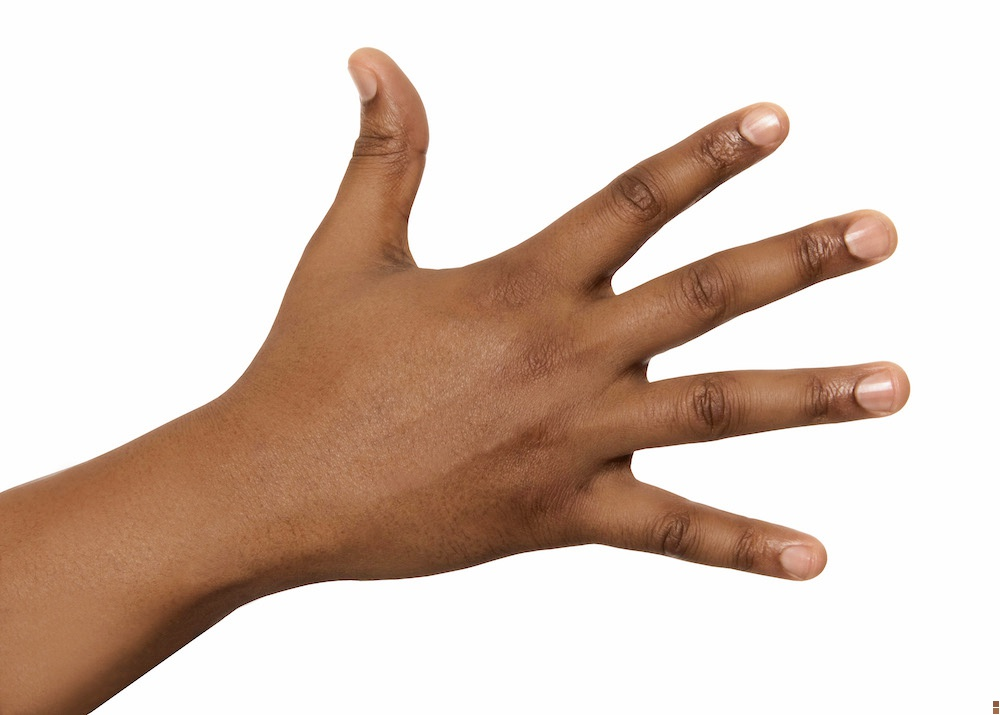
\includegraphics[width=\textwidth,height=\textheight,keepaspectratio]{../rc_test/outputs/20170516_proportional_test/hand_dark_to_hand_brown.jpg}
  \end{minipage} \\
\hline  \label{row:prop_test_1} &
  \begin{minipage}{.29\textwidth}
    \includegraphics[width=\textwidth,height=\textheight,keepaspectratio]{../inputs/hand_dark.jpg}
  \end{minipage} & 
  \begin{minipage}{.29\textwidth}
    \includegraphics[width=\textwidth,height=\textheight,keepaspectratio]{../inputs/hand_light.jpg}
  \end{minipage} & 
  \begin{minipage}{.29\textwidth}
    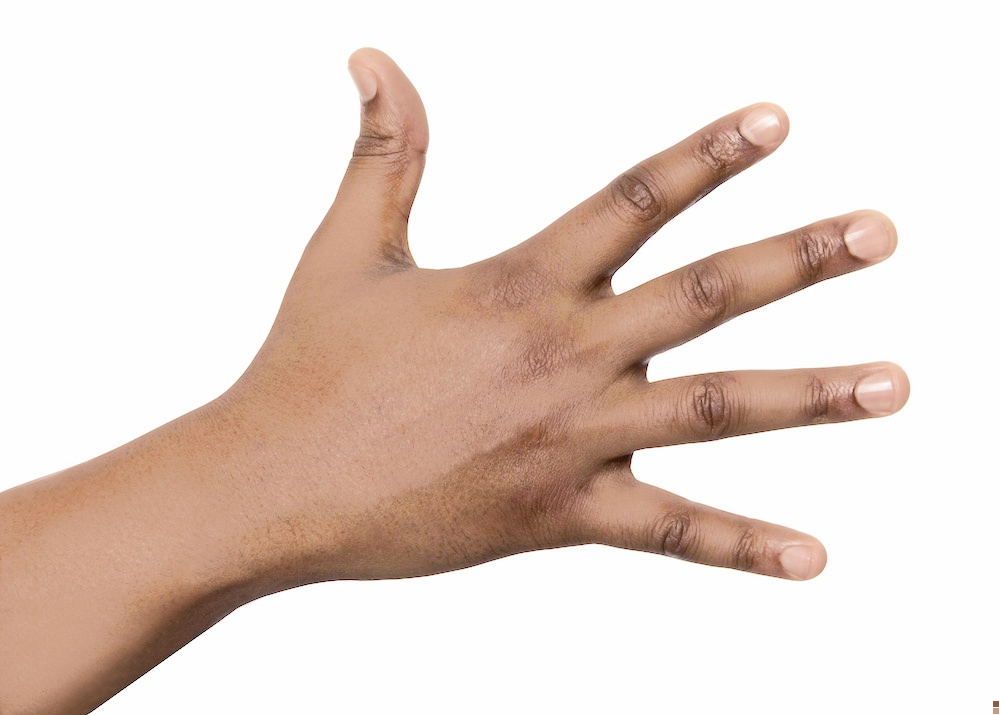
\includegraphics[width=\textwidth,height=\textheight,keepaspectratio]{../rc_test/outputs/20170516_proportional_test/hand_dark_to_hand_light.jpg}
  \end{minipage} \\
\hline  \label{row:prop_test_1} &
  \begin{minipage}{.29\textwidth}
    \includegraphics[width=\textwidth,height=\textheight,keepaspectratio]{../inputs/hand_dark.jpg}
  \end{minipage} & 
  \begin{minipage}{.29\textwidth}
    \includegraphics[width=\textwidth,height=\textheight,keepaspectratio]{../inputs/hand_pale.jpg}
  \end{minipage} & 
  \begin{minipage}{.29\textwidth}
    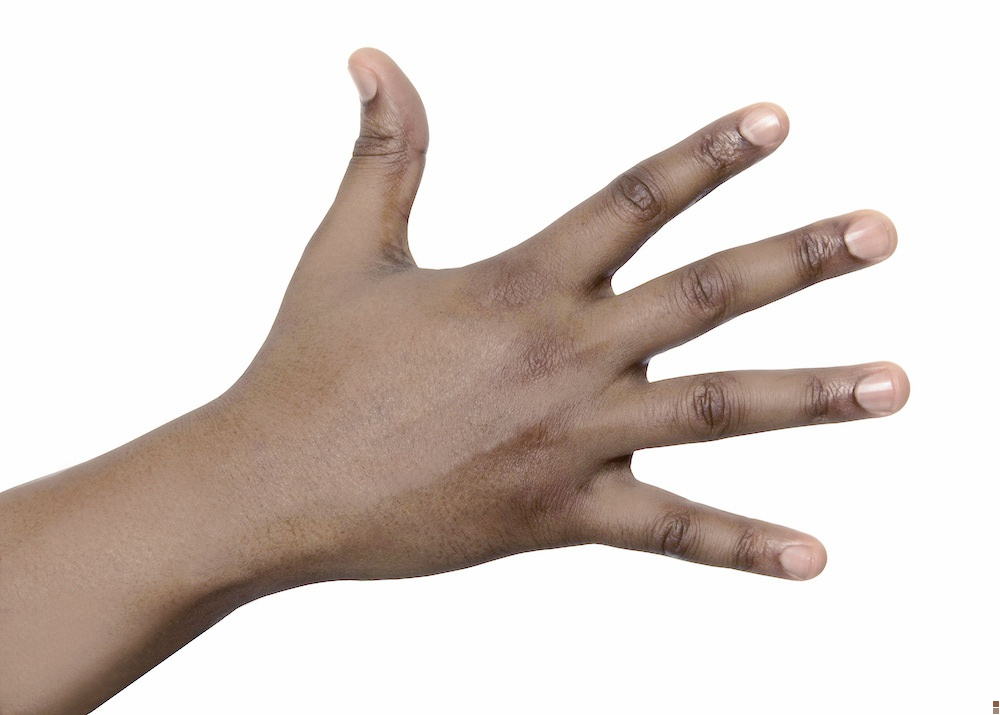
\includegraphics[width=\textwidth,height=\textheight,keepaspectratio]{../rc_test/outputs/20170516_proportional_test/hand_dark_to_hand_pale.jpg}
  \end{minipage} \\
\hline  \label{row:prop_test_1} &
  \begin{minipage}{.29\textwidth}
    \includegraphics[width=\textwidth,height=\textheight,keepaspectratio]{../inputs/hand_brown.jpg}
  \end{minipage} & 
  \begin{minipage}{.29\textwidth}
    \includegraphics[width=\textwidth,height=\textheight,keepaspectratio]{../inputs/hand_dark.jpg}
  \end{minipage} & 
  \begin{minipage}{.29\textwidth}
    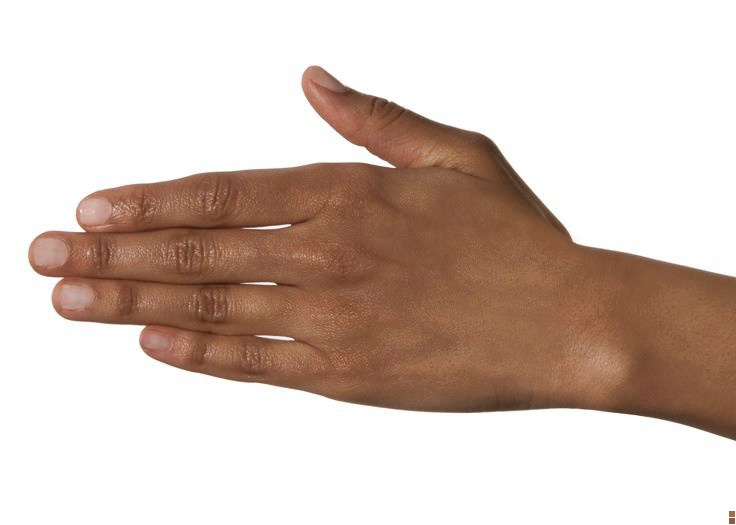
\includegraphics[width=\textwidth,height=\textheight,keepaspectratio]{../rc_test/outputs/20170516_proportional_test/hand_brown_to_hand_dark.jpg}
  \end{minipage} \\
\hline  \label{row:prop_test_1} &
  \begin{minipage}{.29\textwidth}
    \includegraphics[width=\textwidth,height=\textheight,keepaspectratio]{../inputs/hand_brown.jpg}
  \end{minipage} & 
  \begin{minipage}{.29\textwidth}
    \includegraphics[width=\textwidth,height=\textheight,keepaspectratio]{../inputs/hand_light.jpg}
  \end{minipage} & 
  \begin{minipage}{.29\textwidth}
    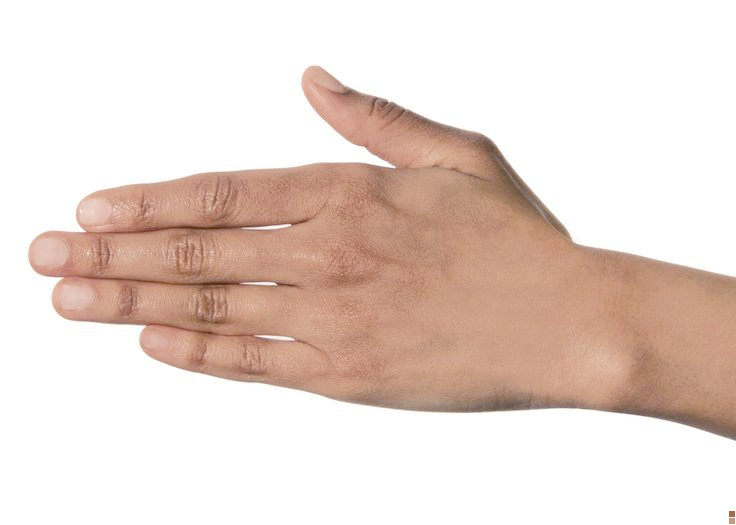
\includegraphics[width=\textwidth,height=\textheight,keepaspectratio]{../rc_test/outputs/20170516_proportional_test/hand_brown_to_hand_light.jpg}
  \end{minipage} \\
\hline  \label{row:prop_test_1} &
  \begin{minipage}{.29\textwidth}
    \includegraphics[width=\textwidth,height=\textheight,keepaspectratio]{../inputs/hand_brown.jpg}
  \end{minipage} & 
  \begin{minipage}{.29\textwidth}
    \includegraphics[width=\textwidth,height=\textheight,keepaspectratio]{../inputs/hand_pale.jpg}
  \end{minipage} & 
  \begin{minipage}{.29\textwidth}
    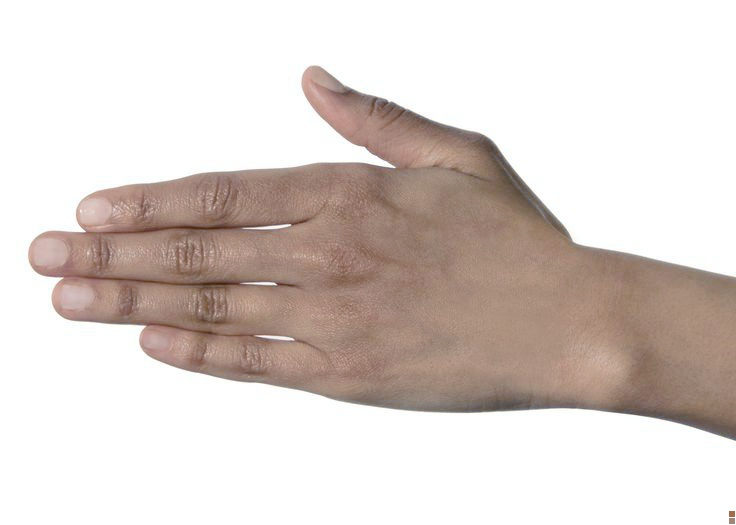
\includegraphics[width=\textwidth,height=\textheight,keepaspectratio]{../rc_test/outputs/20170516_proportional_test/hand_brown_to_hand_pale.jpg}
  \end{minipage} \\
\hline  \label{row:prop_test_1} &
  \begin{minipage}{.29\textwidth}
    \includegraphics[width=\textwidth,height=\textheight,keepaspectratio]{../inputs/hand_light.jpg}
  \end{minipage} & 
  \begin{minipage}{.29\textwidth}
    \includegraphics[width=\textwidth,height=\textheight,keepaspectratio]{../inputs/hand_dark.jpg}
  \end{minipage} & 
  \begin{minipage}{.29\textwidth}
    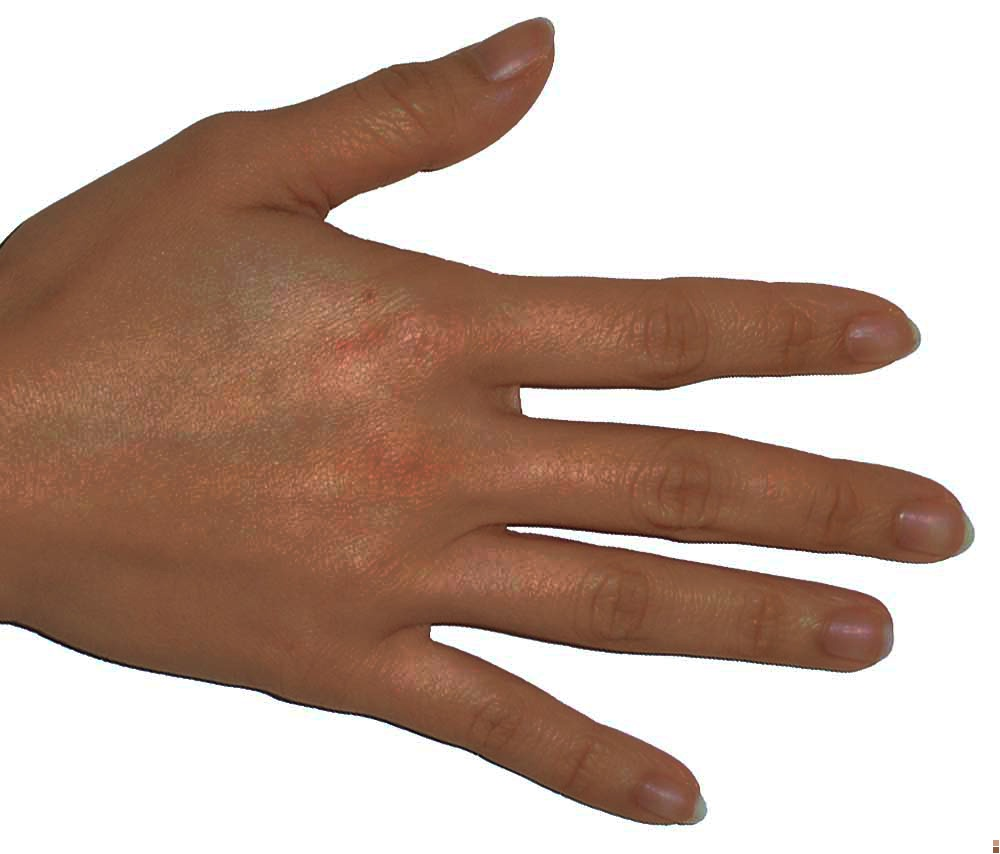
\includegraphics[width=\textwidth,height=\textheight,keepaspectratio]{../rc_test/outputs/20170516_proportional_test/hand_light_to_hand_dark.jpg}
  \end{minipage} \\
\hline  \label{row:prop_test_1} &
  \begin{minipage}{.29\textwidth}
    \includegraphics[width=\textwidth,height=\textheight,keepaspectratio]{../inputs/hand_light.jpg}
  \end{minipage} & 
  \begin{minipage}{.29\textwidth}
    \includegraphics[width=\textwidth,height=\textheight,keepaspectratio]{../inputs/hand_brown.jpg}
  \end{minipage} & 
  \begin{minipage}{.29\textwidth}
    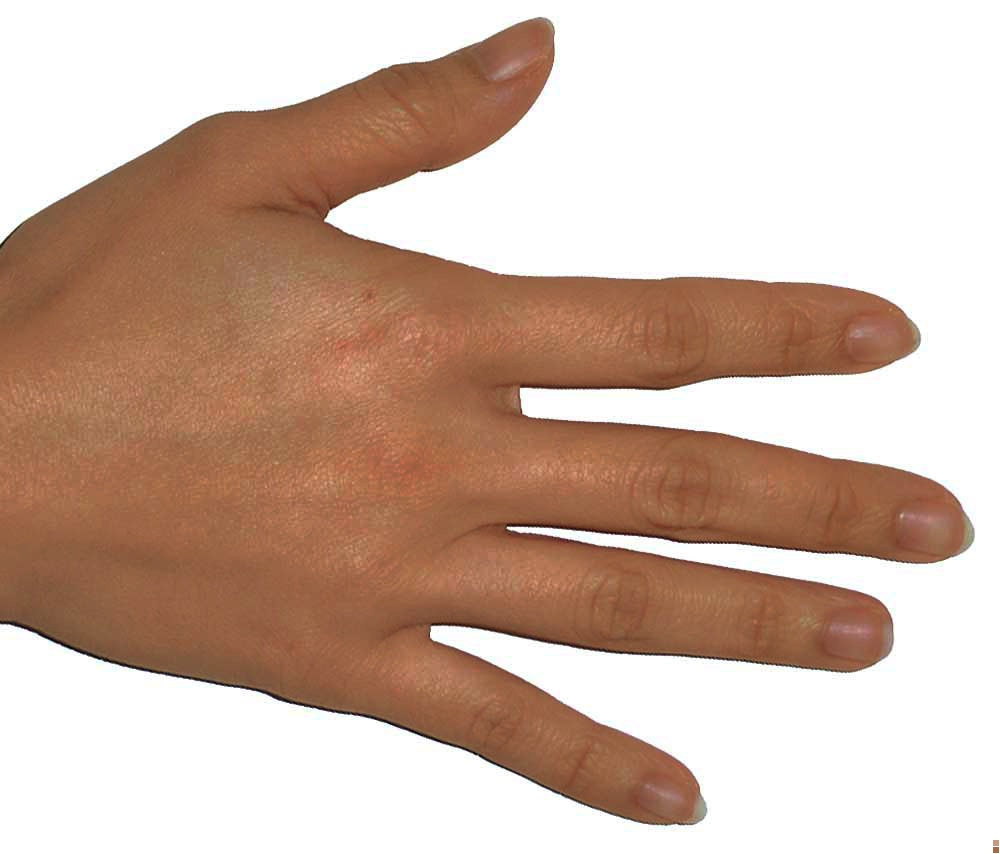
\includegraphics[width=\textwidth,height=\textheight,keepaspectratio]{../rc_test/outputs/20170516_proportional_test/hand_light_to_hand_brown.jpg}
  \end{minipage} \\
\hline  \label{row:prop_test_1} &
  \begin{minipage}{.29\textwidth}
    \includegraphics[width=\textwidth,height=\textheight,keepaspectratio]{../inputs/hand_light.jpg}
  \end{minipage} & 
  \begin{minipage}{.29\textwidth}
    \includegraphics[width=\textwidth,height=\textheight,keepaspectratio]{../inputs/hand_pale.jpg}
  \end{minipage} & 
  \begin{minipage}{.29\textwidth}
    \includegraphics[width=\textwidth,height=\textheight,keepaspectratio]{../rc_test/outputs/20170516_proportional_test/hand_light_to_hand_pale.jpg}
  \end{minipage} \\
\hline  \label{row:prop_test_1} &
  \begin{minipage}{.29\textwidth}
    \includegraphics[width=\textwidth,height=\textheight,keepaspectratio]{../inputs/hand_pale.jpg}
  \end{minipage} & 
  \begin{minipage}{.29\textwidth}
    \includegraphics[width=\textwidth,height=\textheight,keepaspectratio]{../inputs/hand_dark.jpg}
  \end{minipage} & 
  \begin{minipage}{.29\textwidth}
    \includegraphics[width=\textwidth,height=\textheight,keepaspectratio]{../rc_test/outputs/20170516_proportional_test/hand_pale_to_hand_dark.jpg}
  \end{minipage} \\
\hline  \label{row:prop_test_1} &
  \begin{minipage}{.29\textwidth}
    \includegraphics[width=\textwidth,height=\textheight,keepaspectratio]{../inputs/hand_pale.jpg}
  \end{minipage} & 
  \begin{minipage}{.29\textwidth}
    \includegraphics[width=\textwidth,height=\textheight,keepaspectratio]{../inputs/hand_brown.jpg}
  \end{minipage} & 
  \begin{minipage}{.29\textwidth}
    \includegraphics[width=\textwidth,height=\textheight,keepaspectratio]{../rc_test/outputs/20170516_proportional_test/hand_pale_to_hand_brown.jpg}
  \end{minipage} \\
\hline  \label{row:prop_test_1} &
  \begin{minipage}{.29\textwidth}
    \includegraphics[width=\textwidth,height=\textheight,keepaspectratio]{../inputs/hand_pale.jpg}
  \end{minipage} & 
  \begin{minipage}{.29\textwidth}
    \includegraphics[width=\textwidth,height=\textheight,keepaspectratio]{../inputs/hand_light.jpg}
  \end{minipage} & 
  \begin{minipage}{.29\textwidth}
    \includegraphics[width=\textwidth,height=\textheight,keepaspectratio]{../rc_test/outputs/20170516_proportional_test/hand_pale_to_hand_light.jpg}
  \end{minipage} \\
\hline
 \end{longtable}
\pagebreak
\begin{longtable}{|N||c|c|c|}
	\caption{Test results of proportional brightening with correction for dark spots\label{tab:prop_correct_test}}\\
	\hline
	\multicolumn{1}{|c||}{No.} & Original & Target & Results \\ 
	\hline
	    \label{row:prop_correct_test_1} &
  \begin{minipage}{.29\textwidth}
    \includegraphics[width=\textwidth,height=\textheight,keepaspectratio]{../inputs/hand_dark.jpg}
  \end{minipage} & 
  \begin{minipage}{.29\textwidth}
    \includegraphics[width=\textwidth,height=\textheight,keepaspectratio]{../inputs/hand_brown.jpg}
  \end{minipage} & 
  \begin{minipage}{.29\textwidth}
    \includegraphics[width=\textwidth,height=\textheight,keepaspectratio]{../rc_test/outputs/20170516_proportional_corrected_test/hand_dark_to_hand_brown.jpg}
  \end{minipage} \\
\hline  \label{row:prop_correct_test_1} &
  \begin{minipage}{.29\textwidth}
    \includegraphics[width=\textwidth,height=\textheight,keepaspectratio]{../inputs/hand_dark.jpg}
  \end{minipage} & 
  \begin{minipage}{.29\textwidth}
    \includegraphics[width=\textwidth,height=\textheight,keepaspectratio]{../inputs/hand_light.jpg}
  \end{minipage} & 
  \begin{minipage}{.29\textwidth}
    \includegraphics[width=\textwidth,height=\textheight,keepaspectratio]{../rc_test/outputs/20170516_proportional_corrected_test/hand_dark_to_hand_light.jpg}
  \end{minipage} \\
\hline  \label{row:prop_correct_test_1} &
  \begin{minipage}{.29\textwidth}
    \includegraphics[width=\textwidth,height=\textheight,keepaspectratio]{../inputs/hand_dark.jpg}
  \end{minipage} & 
  \begin{minipage}{.29\textwidth}
    \includegraphics[width=\textwidth,height=\textheight,keepaspectratio]{../inputs/hand_pale.jpg}
  \end{minipage} & 
  \begin{minipage}{.29\textwidth}
    \includegraphics[width=\textwidth,height=\textheight,keepaspectratio]{../rc_test/outputs/20170516_proportional_corrected_test/hand_dark_to_hand_pale.jpg}
  \end{minipage} \\
\hline  \label{row:prop_correct_test_1} &
  \begin{minipage}{.29\textwidth}
    \includegraphics[width=\textwidth,height=\textheight,keepaspectratio]{../inputs/hand_brown.jpg}
  \end{minipage} & 
  \begin{minipage}{.29\textwidth}
    \includegraphics[width=\textwidth,height=\textheight,keepaspectratio]{../inputs/hand_dark.jpg}
  \end{minipage} & 
  \begin{minipage}{.29\textwidth}
    \includegraphics[width=\textwidth,height=\textheight,keepaspectratio]{../rc_test/outputs/20170516_proportional_corrected_test/hand_brown_to_hand_dark.jpg}
  \end{minipage} \\
\hline  \label{row:prop_correct_test_1} &
  \begin{minipage}{.29\textwidth}
    \includegraphics[width=\textwidth,height=\textheight,keepaspectratio]{../inputs/hand_brown.jpg}
  \end{minipage} & 
  \begin{minipage}{.29\textwidth}
    \includegraphics[width=\textwidth,height=\textheight,keepaspectratio]{../inputs/hand_light.jpg}
  \end{minipage} & 
  \begin{minipage}{.29\textwidth}
    \includegraphics[width=\textwidth,height=\textheight,keepaspectratio]{../rc_test/outputs/20170516_proportional_corrected_test/hand_brown_to_hand_light.jpg}
  \end{minipage} \\
\hline  \label{row:prop_correct_test_1} &
  \begin{minipage}{.29\textwidth}
    \includegraphics[width=\textwidth,height=\textheight,keepaspectratio]{../inputs/hand_brown.jpg}
  \end{minipage} & 
  \begin{minipage}{.29\textwidth}
    \includegraphics[width=\textwidth,height=\textheight,keepaspectratio]{../inputs/hand_pale.jpg}
  \end{minipage} & 
  \begin{minipage}{.29\textwidth}
    \includegraphics[width=\textwidth,height=\textheight,keepaspectratio]{../rc_test/outputs/20170516_proportional_corrected_test/hand_brown_to_hand_pale.jpg}
  \end{minipage} \\
\hline  \label{row:prop_correct_test_1} &
  \begin{minipage}{.29\textwidth}
    \includegraphics[width=\textwidth,height=\textheight,keepaspectratio]{../inputs/hand_light.jpg}
  \end{minipage} & 
  \begin{minipage}{.29\textwidth}
    \includegraphics[width=\textwidth,height=\textheight,keepaspectratio]{../inputs/hand_dark.jpg}
  \end{minipage} & 
  \begin{minipage}{.29\textwidth}
    \includegraphics[width=\textwidth,height=\textheight,keepaspectratio]{../rc_test/outputs/20170516_proportional_corrected_test/hand_light_to_hand_dark.jpg}
  \end{minipage} \\
\hline  \label{row:prop_correct_test_1} &
  \begin{minipage}{.29\textwidth}
    \includegraphics[width=\textwidth,height=\textheight,keepaspectratio]{../inputs/hand_light.jpg}
  \end{minipage} & 
  \begin{minipage}{.29\textwidth}
    \includegraphics[width=\textwidth,height=\textheight,keepaspectratio]{../inputs/hand_brown.jpg}
  \end{minipage} & 
  \begin{minipage}{.29\textwidth}
    \includegraphics[width=\textwidth,height=\textheight,keepaspectratio]{../rc_test/outputs/20170516_proportional_corrected_test/hand_light_to_hand_brown.jpg}
  \end{minipage} \\
\hline  \label{row:prop_correct_test_1} &
  \begin{minipage}{.29\textwidth}
    \includegraphics[width=\textwidth,height=\textheight,keepaspectratio]{../inputs/hand_light.jpg}
  \end{minipage} & 
  \begin{minipage}{.29\textwidth}
    \includegraphics[width=\textwidth,height=\textheight,keepaspectratio]{../inputs/hand_pale.jpg}
  \end{minipage} & 
  \begin{minipage}{.29\textwidth}
    \includegraphics[width=\textwidth,height=\textheight,keepaspectratio]{../rc_test/outputs/20170516_proportional_corrected_test/hand_light_to_hand_pale.jpg}
  \end{minipage} \\
\hline  \label{row:prop_correct_test_1} &
  \begin{minipage}{.29\textwidth}
    \includegraphics[width=\textwidth,height=\textheight,keepaspectratio]{../inputs/hand_pale.jpg}
  \end{minipage} & 
  \begin{minipage}{.29\textwidth}
    \includegraphics[width=\textwidth,height=\textheight,keepaspectratio]{../inputs/hand_dark.jpg}
  \end{minipage} & 
  \begin{minipage}{.29\textwidth}
    \includegraphics[width=\textwidth,height=\textheight,keepaspectratio]{../rc_test/outputs/20170516_proportional_corrected_test/hand_pale_to_hand_dark.jpg}
  \end{minipage} \\
\hline  \label{row:prop_correct_test_1} &
  \begin{minipage}{.29\textwidth}
    \includegraphics[width=\textwidth,height=\textheight,keepaspectratio]{../inputs/hand_pale.jpg}
  \end{minipage} & 
  \begin{minipage}{.29\textwidth}
    \includegraphics[width=\textwidth,height=\textheight,keepaspectratio]{../inputs/hand_brown.jpg}
  \end{minipage} & 
  \begin{minipage}{.29\textwidth}
    \includegraphics[width=\textwidth,height=\textheight,keepaspectratio]{../rc_test/outputs/20170516_proportional_corrected_test/hand_pale_to_hand_brown.jpg}
  \end{minipage} \\
\hline  \label{row:prop_correct_test_1} &
  \begin{minipage}{.29\textwidth}
    \includegraphics[width=\textwidth,height=\textheight,keepaspectratio]{../inputs/hand_pale.jpg}
  \end{minipage} & 
  \begin{minipage}{.29\textwidth}
    \includegraphics[width=\textwidth,height=\textheight,keepaspectratio]{../inputs/hand_light.jpg}
  \end{minipage} & 
  \begin{minipage}{.29\textwidth}
    \includegraphics[width=\textwidth,height=\textheight,keepaspectratio]{../rc_test/outputs/20170516_proportional_corrected_test/hand_pale_to_hand_light.jpg}
  \end{minipage} \\
\hline
 \end{longtable}

\end{document}